\chapter{Methods}
\label{chap:methods}
\TODO{Intro - of chapter and probably other chapter name}\\
To train any kind of statistical or machine learning model we need a large enough dataset. For our initial studies we will use various subsets of the QM9 dataset \parencite{ref:article1_qm9, ref:article2_qm9}. \TODO{More intro \& reference to Background chapter}

\section{QM9 dataset \parencite{ref:data_qm9}}
\label{sec:qm9}
Time savings given through faster convergence are especially relevant for larger systems where the number of SCF iterations are and especially the number of integrals to be calculated are large. Stated differently, it is of little interest to optimize guessing methods for small systems which converge in a near instantly on conventional hardware. Furthermore, a constant input and output size is required to train most machine learning models. \\
The QM9 dataset \parencite{ref:article1_qm9,ref:article2_qm9} ticks both of these two boxes. It offers a diverse variety of molecules from as little as 3 constituent atoms up to 29 atoms. Additionally, there are large enough chunks of constitutional isomers to train models on these subsets of same sized matrices. 
\begin{figure}[H]
    \centering
    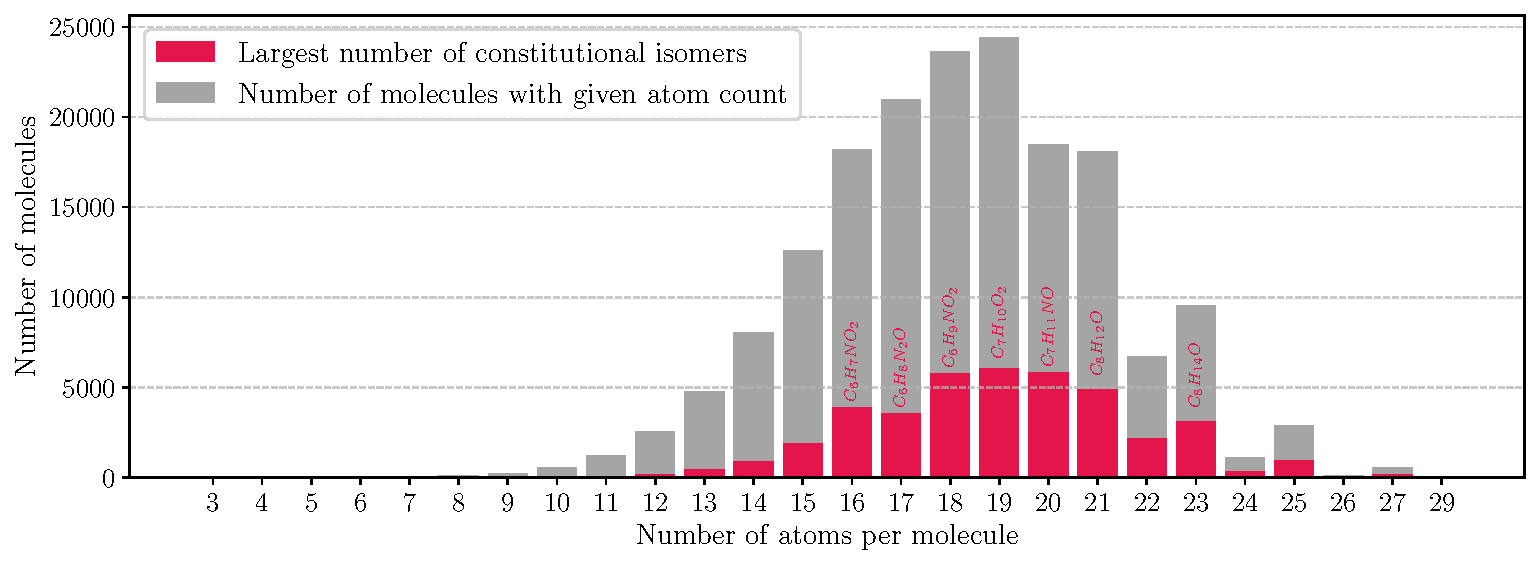
\includegraphics[width=\textwidth]{../fig/qm9_general/qm9_overview_stacked_bar.pdf}
    \caption[QM9 dataset overview]{Overview of the QM9 dataset. The dataset contains 134k molecules with up to nine heavy - \ch{C} \ch{O} \ch{N} \ch{F} - atoms. Large groups of constitutional isomers are present (largest depicted in red). The properties are calculated using DFT with the B3LYP functional and the 6-31G(2df,p) basis set.}
    \label{fig:method_qm9_overview}
\end{figure}


\section{Fock Matrix prediction: A first trial}
\label{sec:first_predictions}
SCF methods by nature initially need a density matrix to start off their iterative calculations. Independent of the way the initial guess is chosen the computational effort of this step should be negligible compared to the actual SCF iterations. 


\subsection{\ch{C5H4N2O2}}

\section{Software and Implementation Specifics}
\label{sec:software_and_implementation}
Reproducability crisis
\section{Cost function}
\section{Dataset}